\documentclass[12pt,a4]{article}
%\usepackage{polski}
\usepackage{fontawesome}
\usepackage[utf8]{inputenc}
%\usepackage{tikz}
\usepackage[table]{xcolor}
\usepackage{enumerate}
\usepackage{graphicx}
\usepackage{float}
\usepackage{subcaption}
\usepackage{array}
\usepackage{amsmath}
\usepackage{amssymb}
\usepackage{mathtools}
\usepackage{tabularx}
\usepackage{physics}
\usepackage{booktabs}
\usepackage{multirow}
\usepackage{multicol}
\usepackage{hyperref}
\usepackage{dsfont}
\usepackage{parskip}
\usepackage{tcolorbox}

\usepackage{geometry}

\newgeometry{tmargin=2cm, bmargin=1.5cm, lmargin=2cm, rmargin=2cm}

\usepackage{sectsty}
\definecolor{ColorOne}{RGB}{53, 78, 140}
\definecolor{AGHgreen}{RGB}{0, 105, 60}
\definecolor{AGHblack}{RGB}{30, 30, 30}
\definecolor{AGHred}{RGB}{167, 25, 48}
\sectionfont{\color{AGHgreen}} 
\subsectionfont{\color{AGHgreen}} 
\subsubsectionfont{\color{AGHgreen}} 
\hypersetup{
	colorlinks=true,
	linkcolor=AGHgreen,
	filecolor=AGHgreen,
	urlcolor=AGHgreen,
	citecolor=AGHgreen,
}


%##########################################################################################
%               MOJE KOMENDY
%##########################################################################################

\newcommand{\ods}{\hspace{6mm}}
\newcommand{\noaka}{\noindent}
\newcommand{\aka}{\hspace{6mm}}
\newcommand{\R}{\mathbb{R}}
\newcommand{\krecha}{\rule{\textwidth}{0.25mm}}
\newcommand{\pol}{\frac{1}{2}}


\newcommand{\stopni}{$^\circ$}

\renewcommand{\arraystretch}{1.2}

%\renewcommand{\toprule}{\hline}
%\renewcommand{\bottomrule}{\hline}
%\renewcommand{\midrule}{\hline}


\graphicspath{{./galeria/}}



\newcommand{\machine}[1]{\textcolor{ColorOne}{\texttt{#1}}}

% draw a frame around given text
\newcommand{\framedtext}[1]{%
\par%
\noindent\fcolorbox{black}{gray!7}{%
    \parbox{\dimexpr\linewidth-2\fboxsep-2\fboxrule}{
    \centering
    \parbox{\dimexpr\linewidth-3mm}{
    \vspace{1mm}
    #1
    \vspace{1mm}
    }
    }%
}%
}

\newcommand{\imptext}[1]{%
\par%
\noindent\fcolorbox{black}{AGHgreen!7}{%
    \parbox{\dimexpr\linewidth-2\fboxsep-2\fboxrule}{
    \centering
    \parbox{\dimexpr\linewidth-3mm}{
    \vspace{1mm}
    #1
    \vspace{1mm}
    }
    }%
}%
}

\newcommand{\boxtext}[1]{%
	\begin{tcolorbox}[colback=gray!15,%gray background
		colframe=gray!15,% black frame colour
		width=\textwidth,% Use 5cm total width,
		arc=3mm, auto outer arc,
		]
		#1
	\end{tcolorbox}
}

\newcommand{\ety}[1]{_{\text{#1}}}
\newcommand{\upety}[1]{^{\text{#1}}}

\newcommand{\wektor}[1]{\left[\begin{array}{c}#1\end{array}\right]}

\newcommand{\der}{\mathrm{d}}

%–––––––––––––––––––––––––––––––––––––––––––––––––––––––
\newcommand{\multiline}[1]{\begin{tabular}{c}
		#1
\end{tabular}}
%–––––––––––––––––––––––––––––––––––––––––––––––––––––––
\newcommand{\doublepage}[2]{
	\noindent
	\begin{minipage}{.49\textwidth}
		#1
	\end{minipage}
	\begin{minipage}{.01\textwidth}
		\hfill
	\end{minipage}
	\begin{minipage}{.49\textwidth}
		#2
	\end{minipage}
	\vspace{1mm}
}
%–––––––––––––––––––––––––––––––––––––––––––––––––––––––




\title{\textsc{Calculating electronic states in 2 dimentional parabolic potential}}
\author{Michał Modrzejewski}
\date{\today}

\begin{document}

\maketitle

\section*{Introduction}

The goal of laboratory class is to calculate the eigenstates and eigenenergies of single electron in two dimentional quantum dot, which is desribed by the parabolic potential
\[\hat{\mathcal{H}} = -\frac{1}{2m*}\left(\pdv[2]{x} + \pdv[2]{y}\right) + \frac{m*}{2} (\omega_x^2 x^2 + \omega_y^2y^2)\]
The generalized hamiltonian eigenproblem is analized using the Gallerkin methon with gaussian functions basis set.

\section*{Results}
\subsection*{Task 1}

In order to properly make use of the Gallerkin method one must be sure, that used basis set is defined correctly. Chosen basis functions are plotted on a figure below:

\begin{figure}[H]
	\begin{subfigure}{0.33\textwidth}
		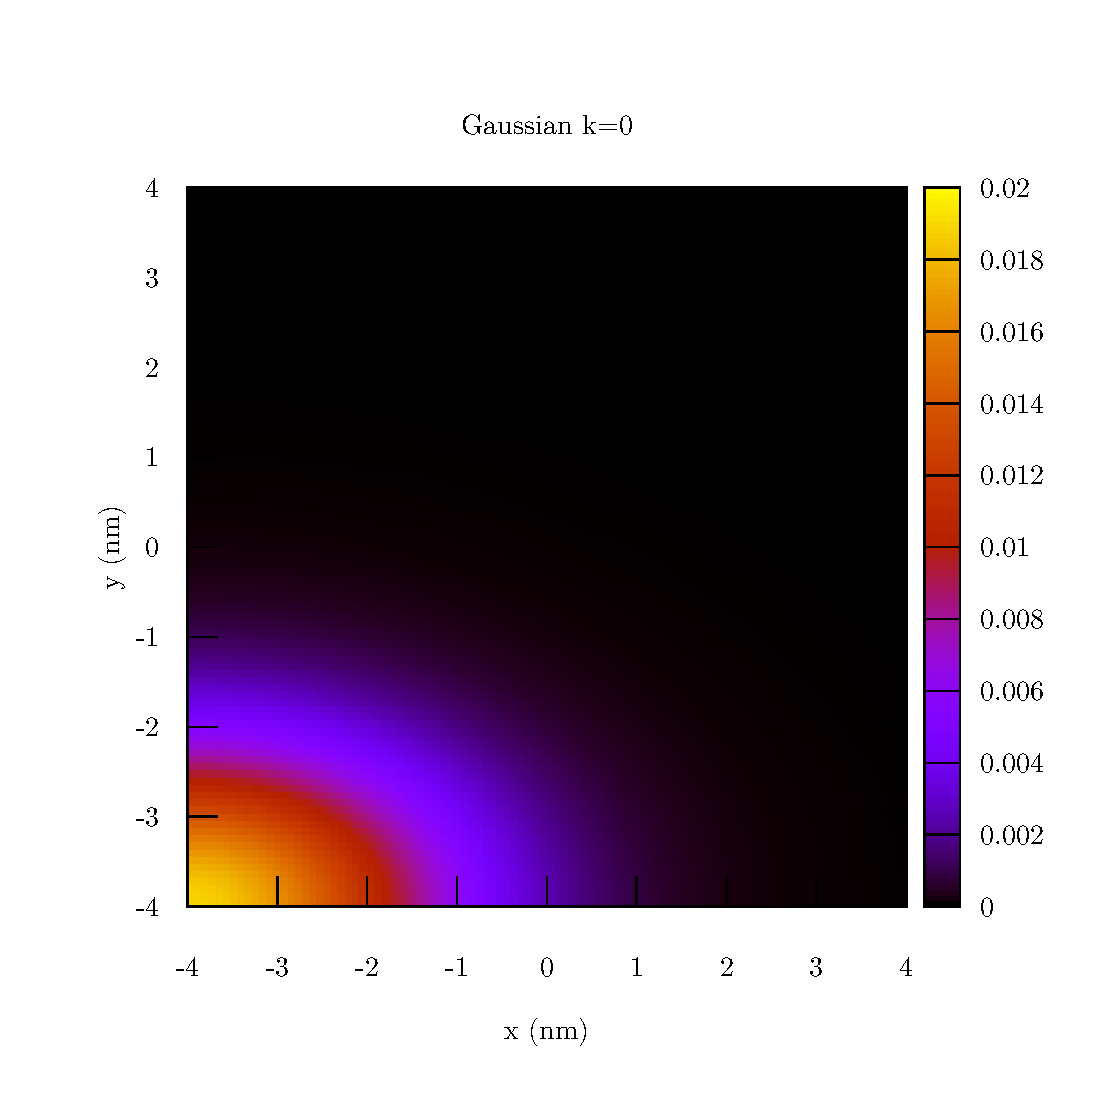
\includegraphics[width=\textwidth]{../plots/basis_0.pdf}
	\end{subfigure}
	\begin{subfigure}{0.33\textwidth}
		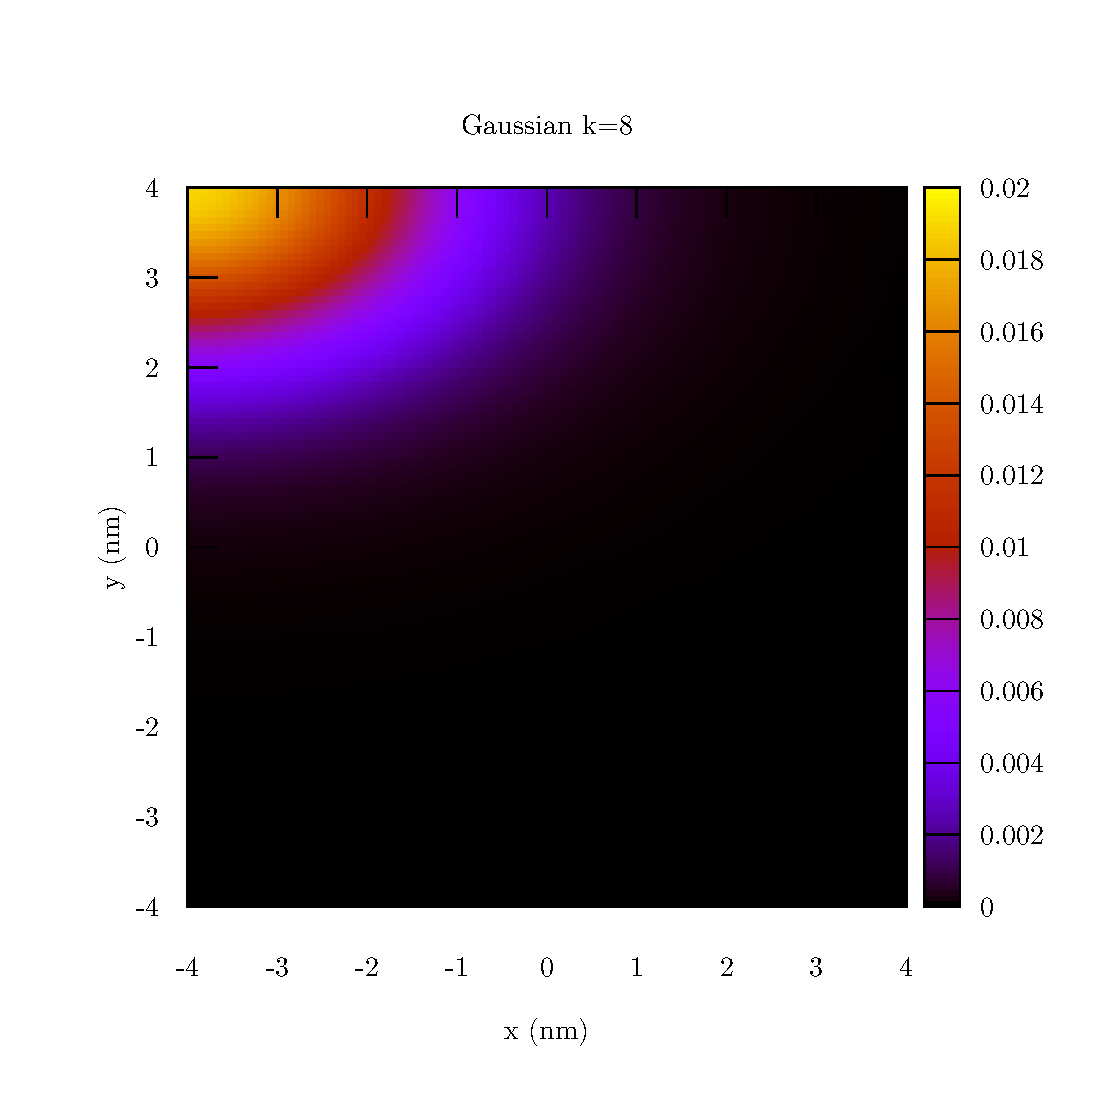
\includegraphics[width=\textwidth]{../plots/basis_8.pdf}
	\end{subfigure}
	\begin{subfigure}{0.33\textwidth}
		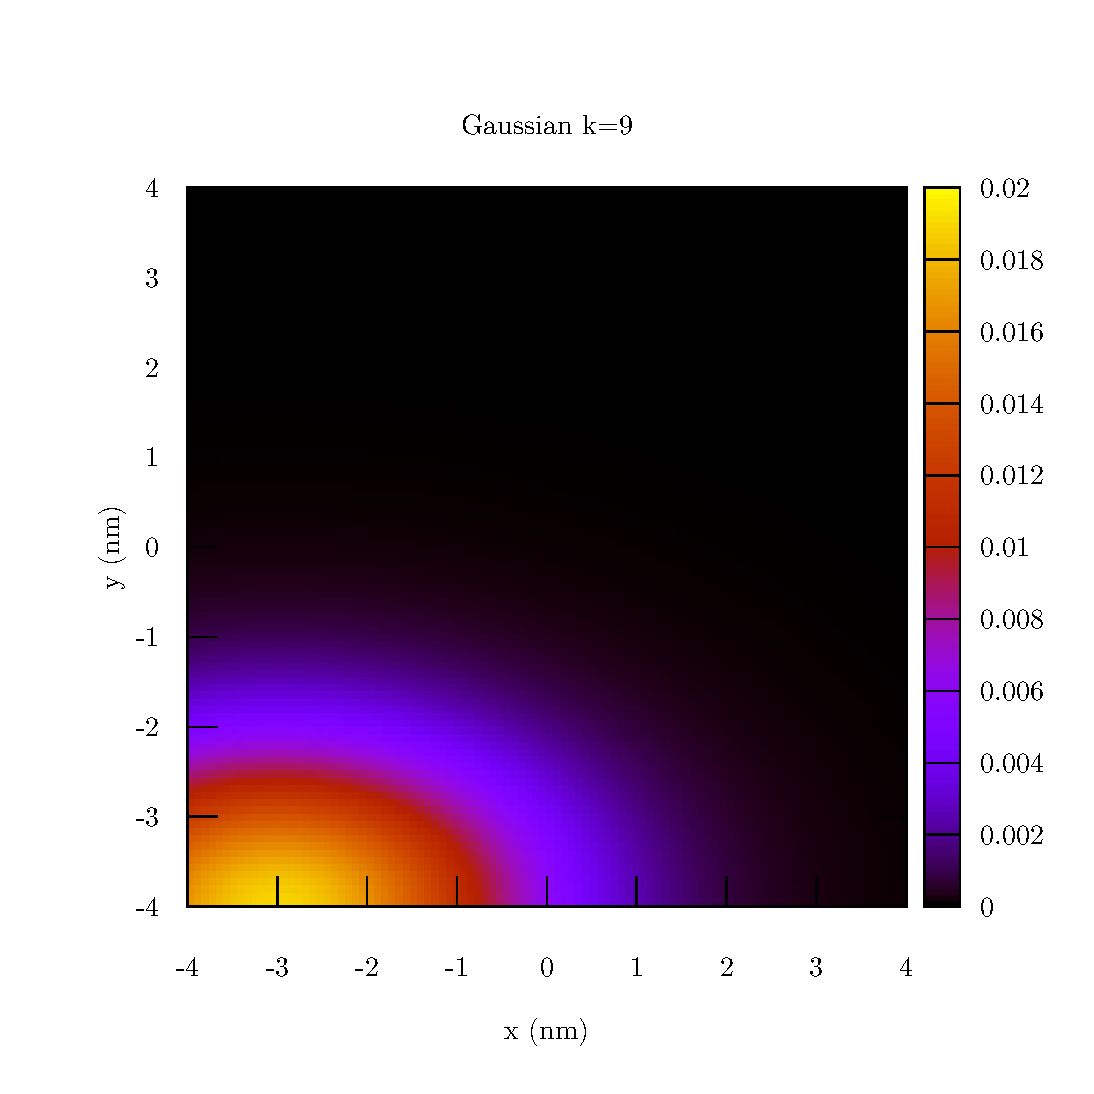
\includegraphics[width=\textwidth]{../plots/basis_9.pdf}
	\end{subfigure}
	\caption{Chosen basis set functions.}
\end{figure}

\subsection*{Task 2}

In order to adress the problem of solving the generalized eigenproblem for analized system a class \texttt{GeneralizedSelfAdjointEigenSolver} from \texttt{C++} library \texttt{Eigen3} was used.

\subsection*{Task 3}

For analized system the squered modulus of the eigenstates wavefunction for 6 lowest energy states were plotted. Said plots are presented on the figure below:

\begin{figure}[H]
	\begin{subfigure}{.33\textwidth}
		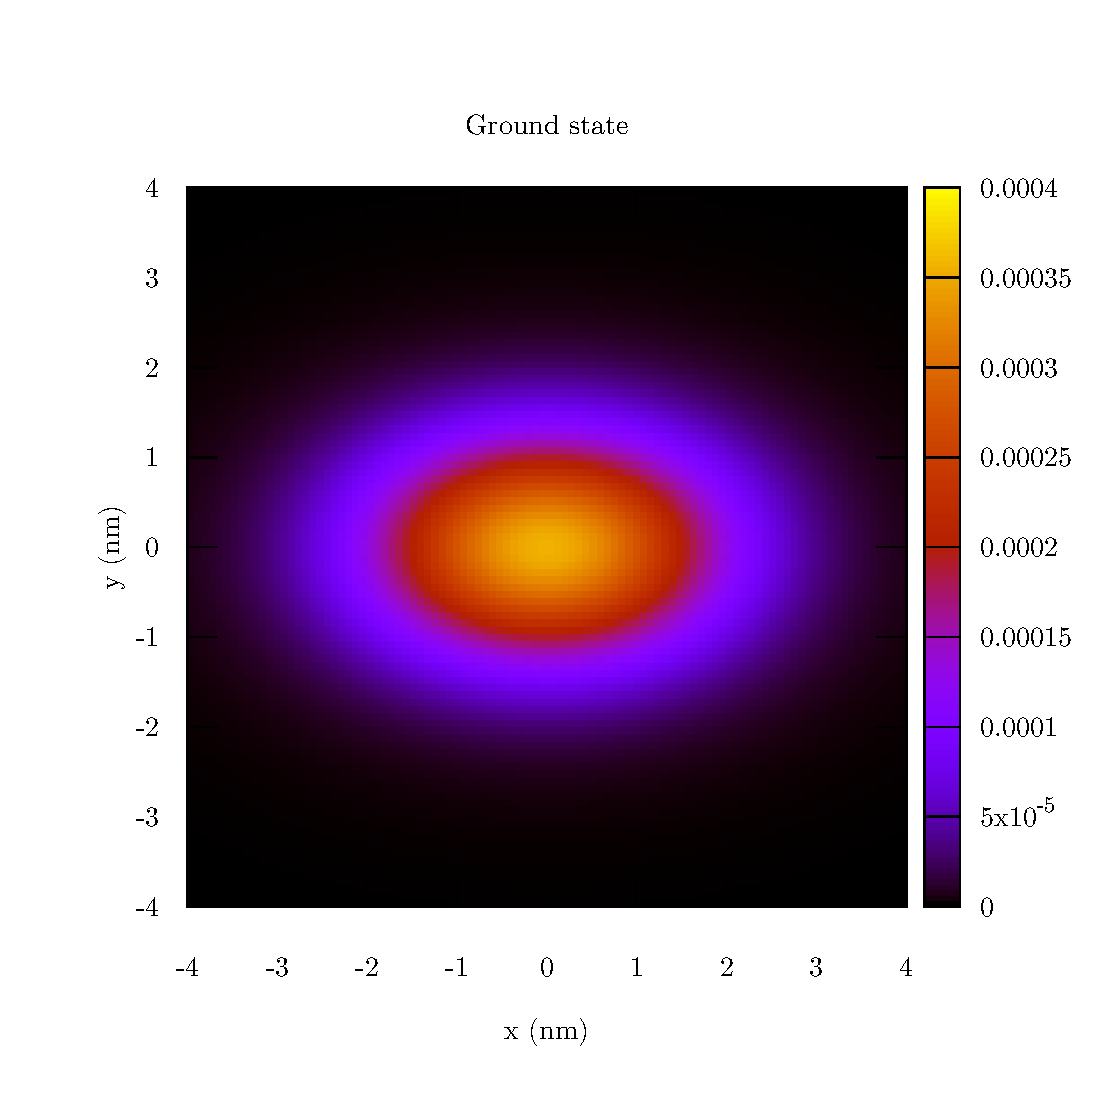
\includegraphics[width=\textwidth]{../plots/state_0.pdf}
		\caption{ground state}
	\end{subfigure}
	\begin{subfigure}{.33\textwidth}
	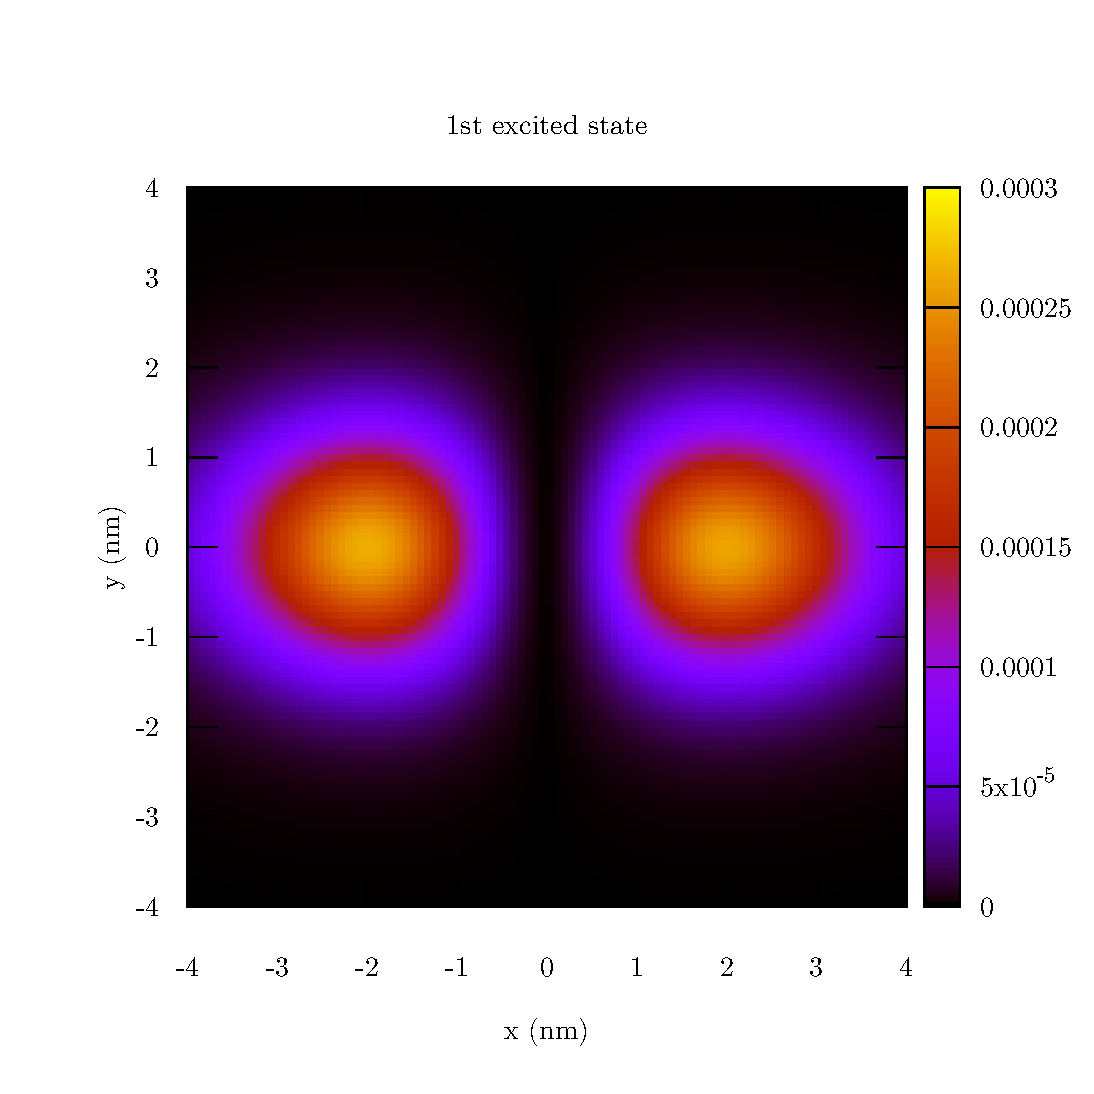
\includegraphics[width=\textwidth]{../plots/state_1.pdf}
	\caption{1st excited state}
	\end{subfigure}
	\begin{subfigure}{.33\textwidth}
	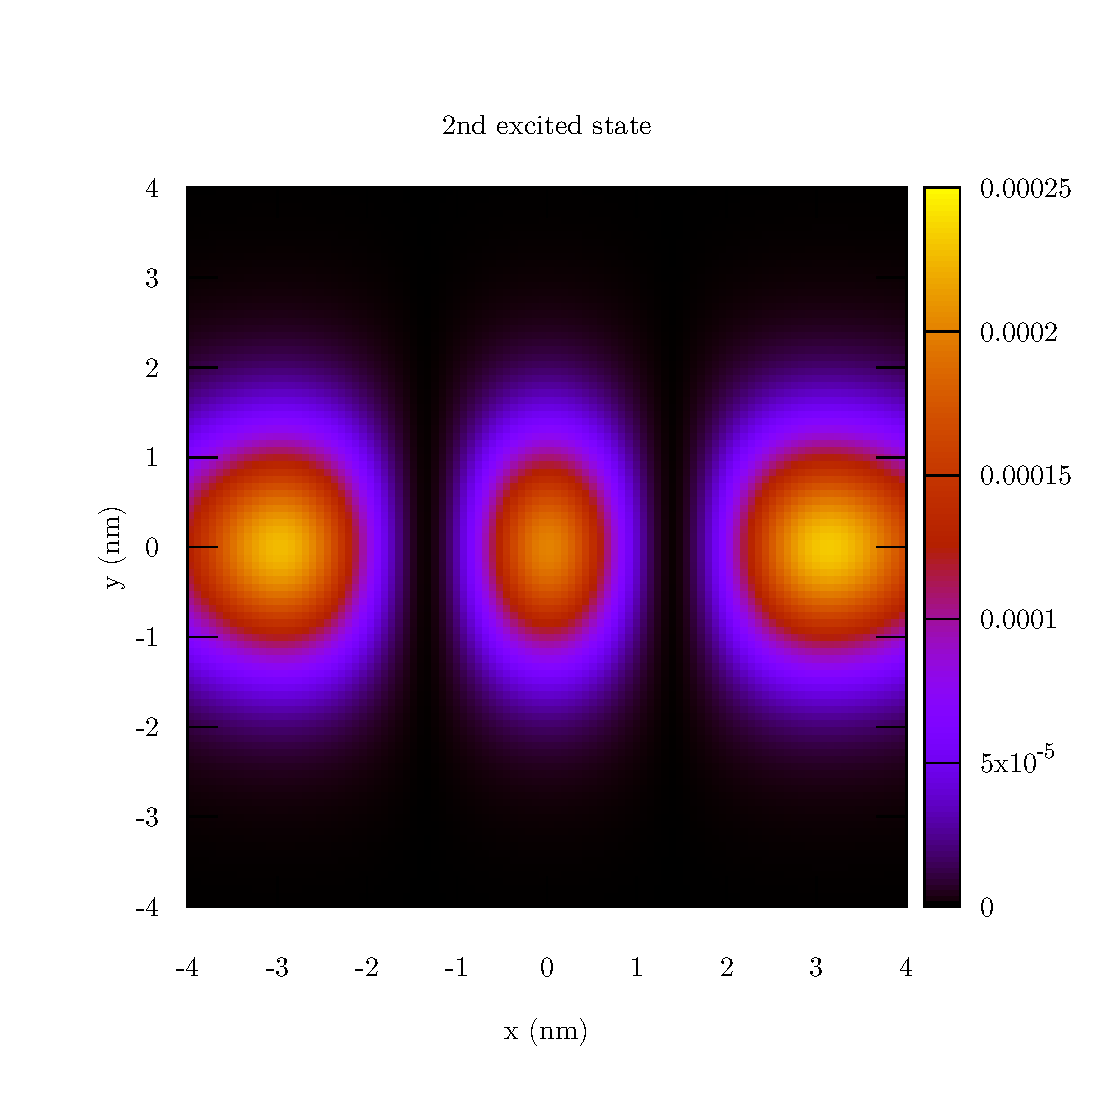
\includegraphics[width=\textwidth]{../plots/state_2.pdf}
	\caption{2nd excited state}
	\end{subfigure}
	\begin{subfigure}{.33\textwidth}
	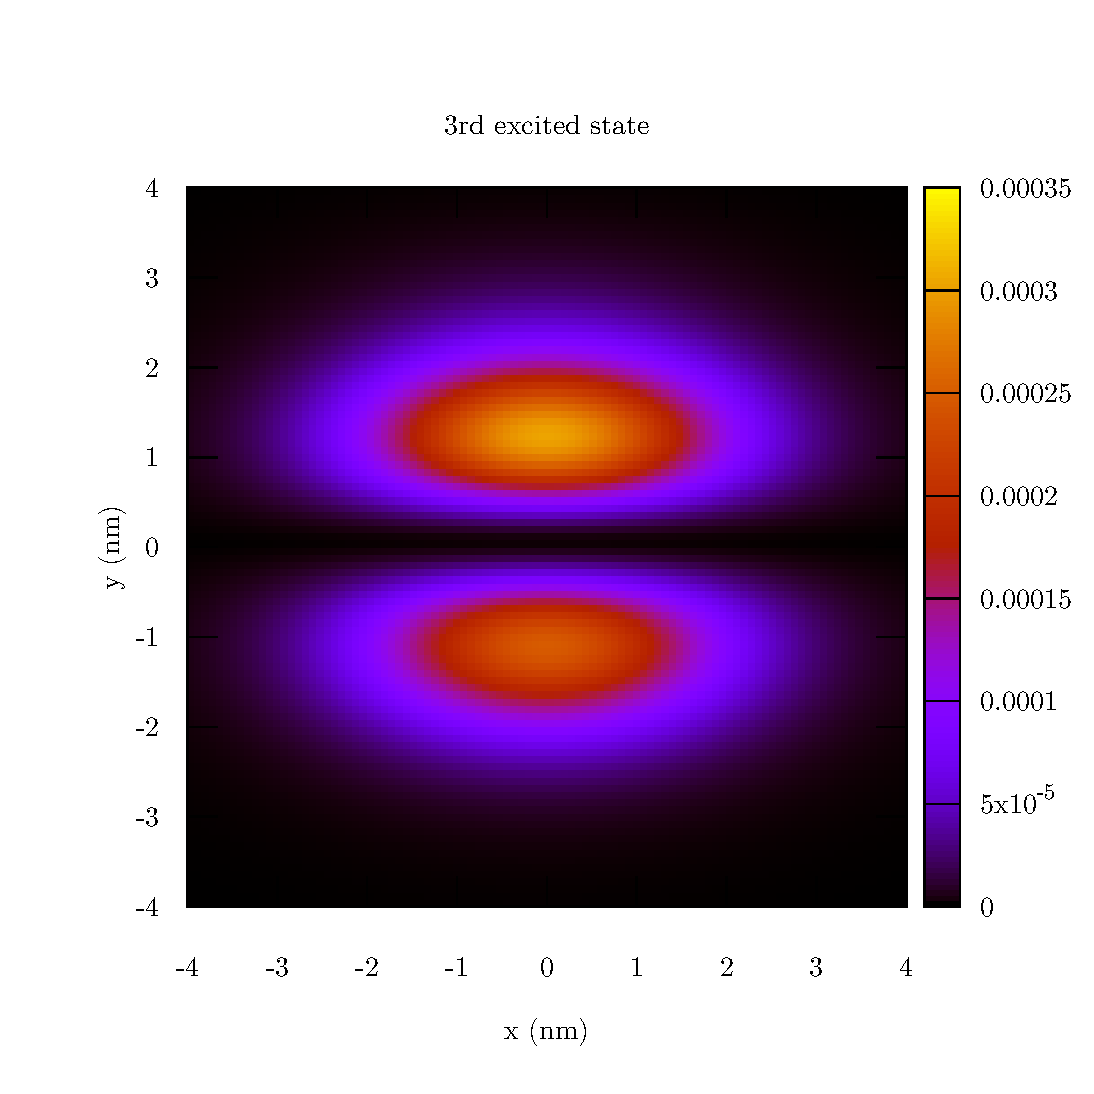
\includegraphics[width=\textwidth]{../plots/state_3.pdf}
	\caption{3rd excited state}
	\end{subfigure}
	\begin{subfigure}{.33\textwidth}
	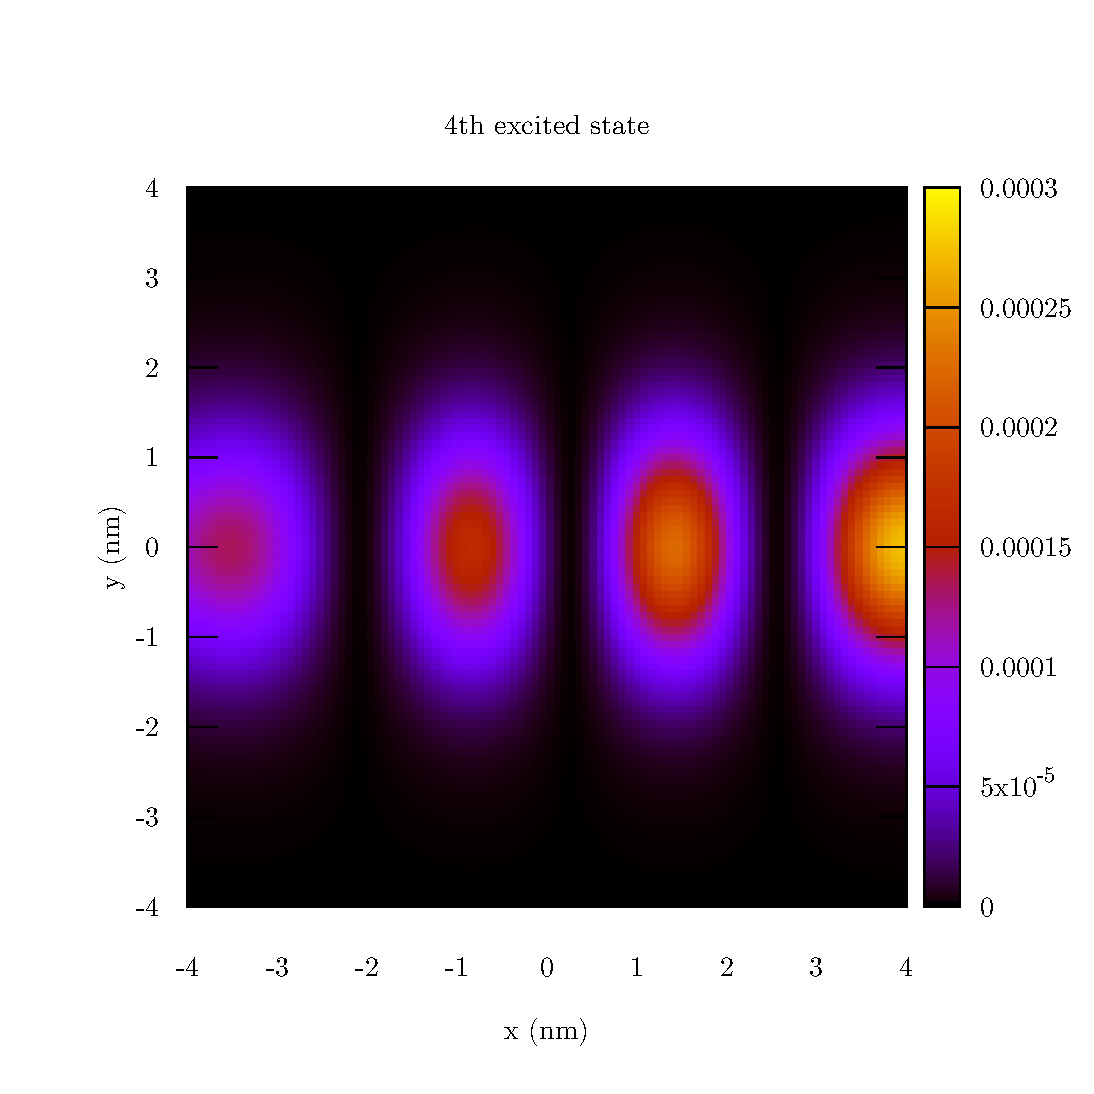
\includegraphics[width=\textwidth]{../plots/state_4.pdf}
	\caption{4th excited state}
	\end{subfigure}
	\begin{subfigure}{.33\textwidth}
	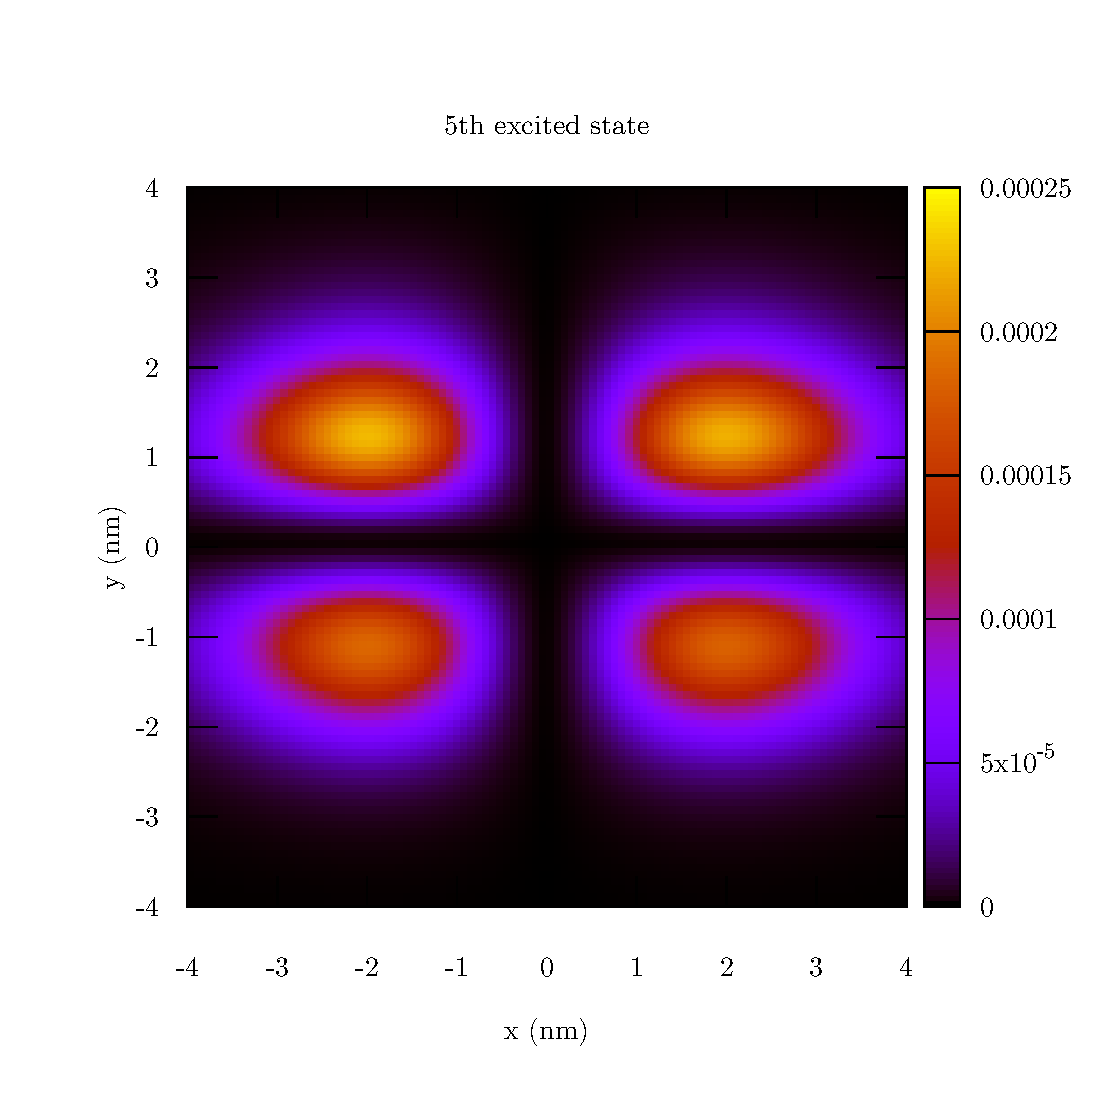
\includegraphics[width=\textwidth]{../plots/state_5.pdf}
	\caption{5th excited state}
	\end{subfigure}
	\caption{Probability densities of eigenstates composed from calculated coefficients for 2D harmonic oscilator.}
\end{figure}

\subsection*{Task 4}

The evolution of eigenenergies for 10 lowest energy states as a function of $ \hbar\omega_x \in [0,500] $ meV is shown on a figure below:

\begin{figure}[H]
	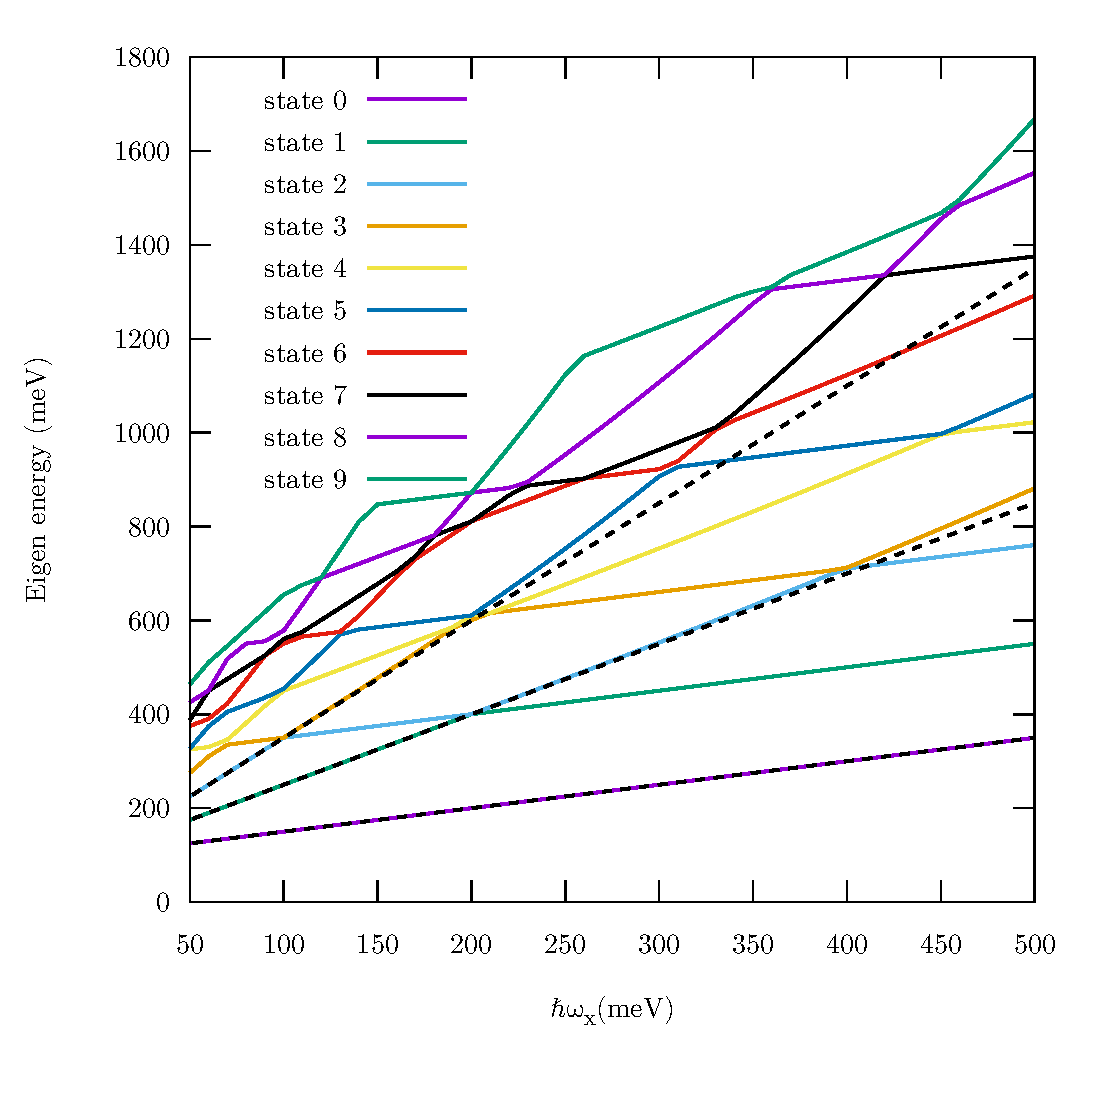
\includegraphics[width=\textwidth]{../plots/E_omega.pdf}
	\caption{10 lowest eigenenergies as a function of $ \hbar\omega_x $ compared with analitical solutions.}
\end{figure}

For higher energies some inaccuracies are visible. Those differences come from small numerical errors, which in accordance to Wilkinson lemat grow and propagate for higher energies. However the calculated groundstate matches perfectly the theoretical value.

\subsection*{Task 5}

The value of $ \hbar\omega_y $ was chosen so that the lowest five states are only excited in the $ x $ direction. Said value was set to $ \hbar\omega_y = 360 $ meV. The plotted probability desities for 5 lowest states can be seen below: 

\begin{figure}[H]
	\begin{subfigure}{.33\textwidth}
		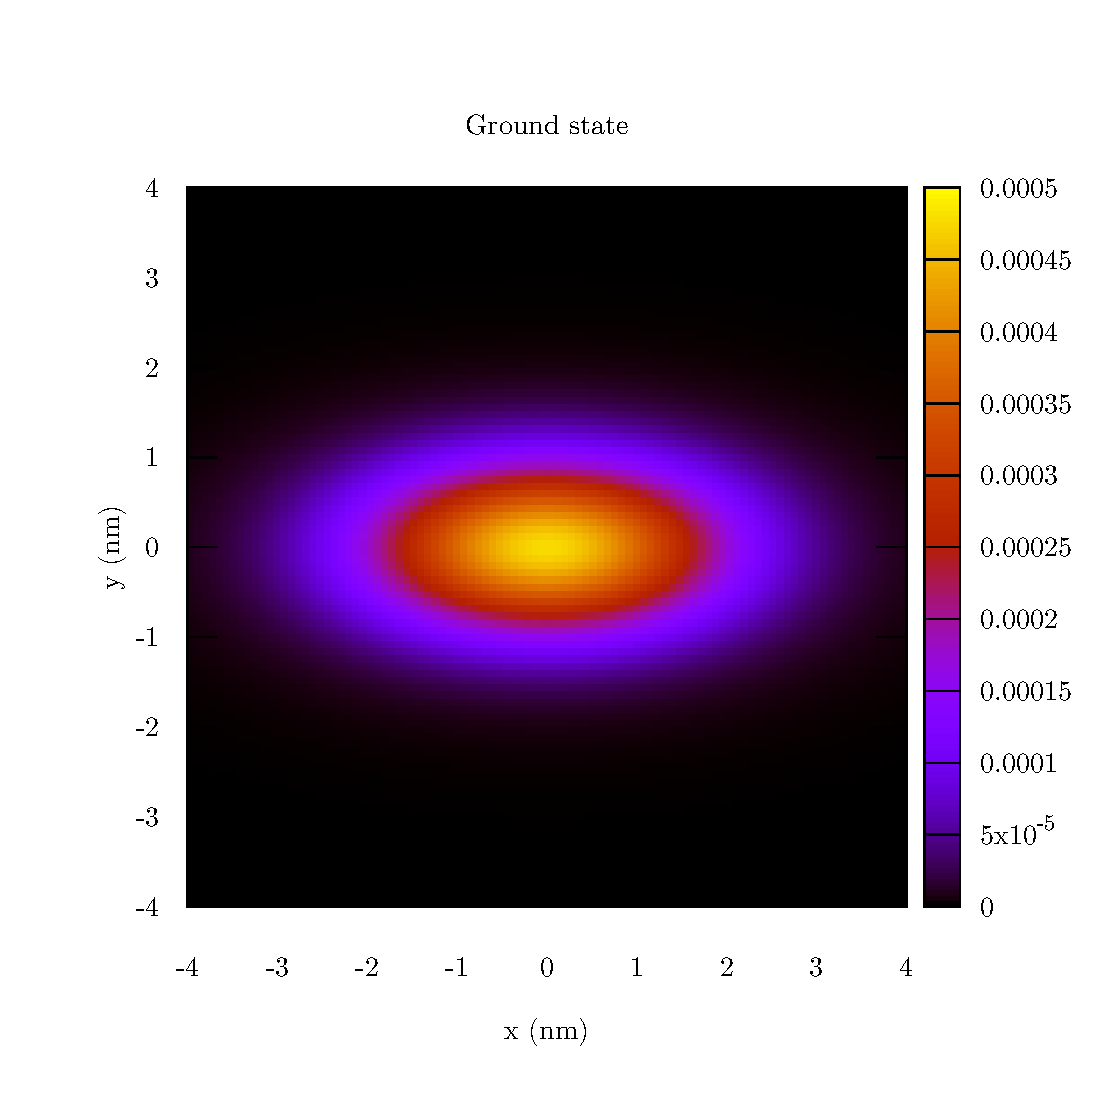
\includegraphics[width=\textwidth]{../plots/y_state_0.pdf}
		\caption{ground state}
	\end{subfigure}
	\begin{subfigure}{.33\textwidth}
		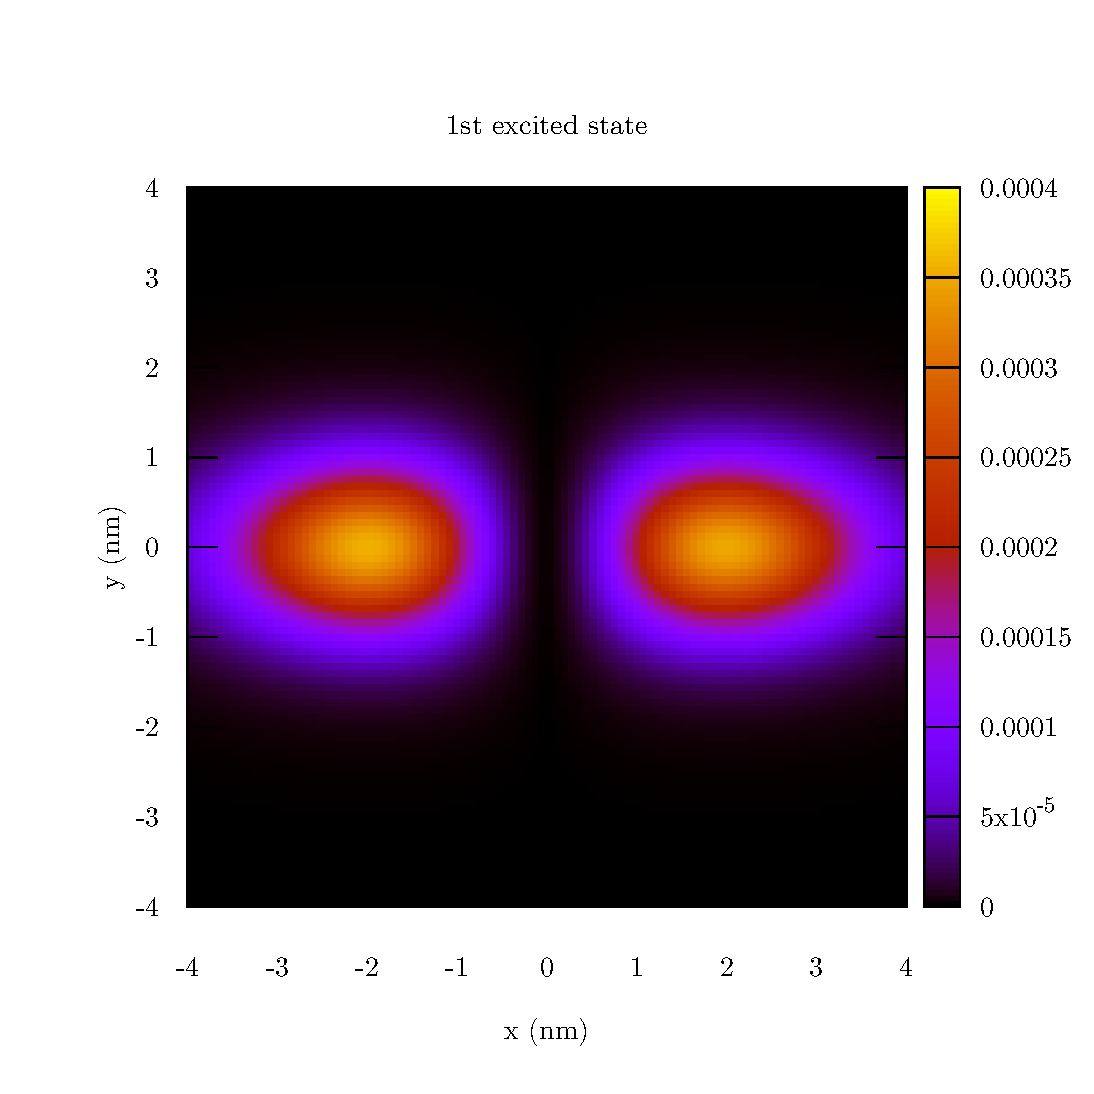
\includegraphics[width=\textwidth]{../plots/y_state_1.pdf}
		\caption{1st excited state}
	\end{subfigure}
	\begin{subfigure}{.33\textwidth}
		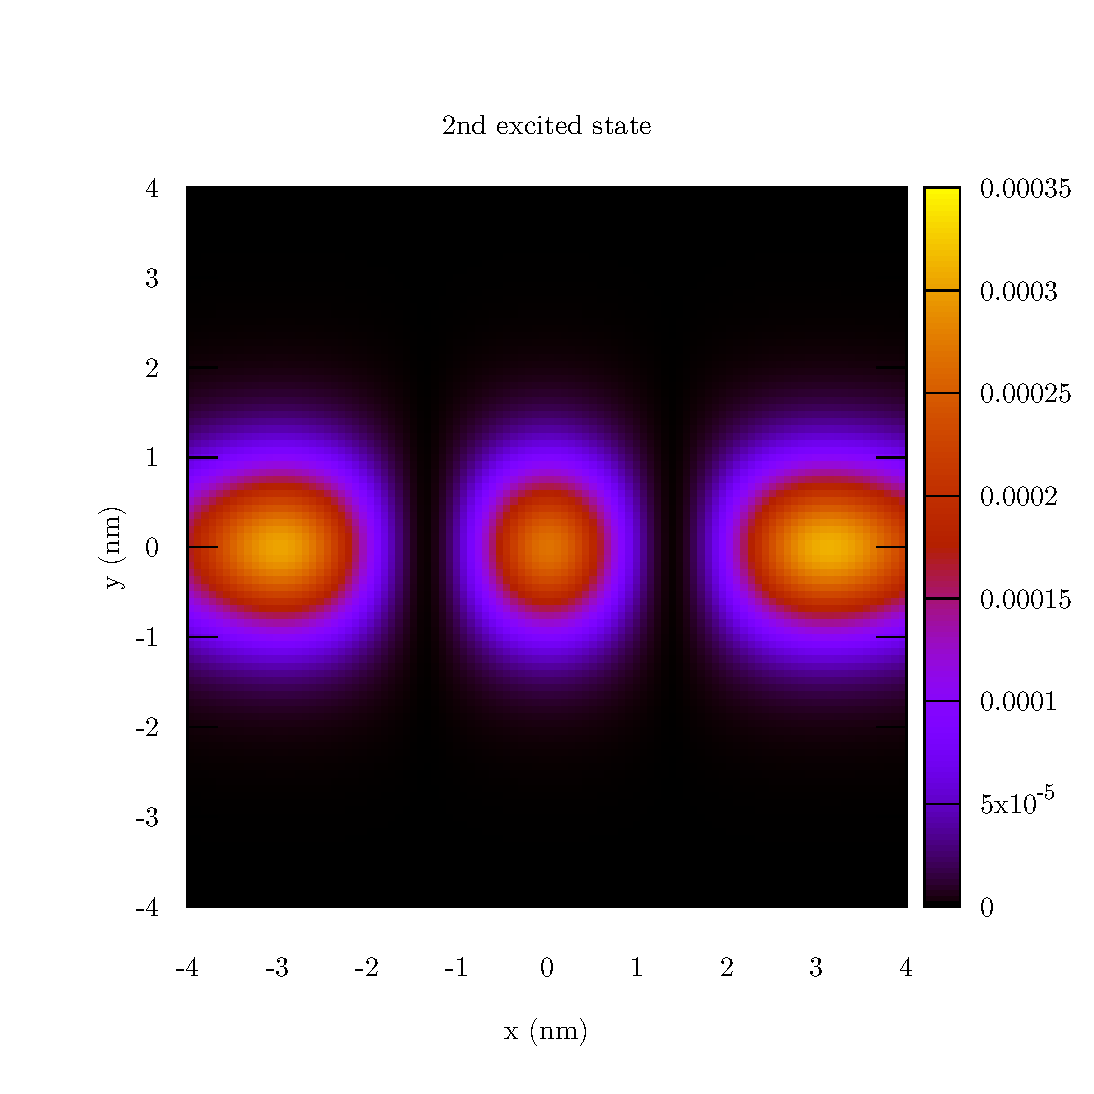
\includegraphics[width=\textwidth]{../plots/y_state_2.pdf}
		\caption{2nd excited state}
	\end{subfigure}
	\begin{subfigure}{.33\textwidth}
		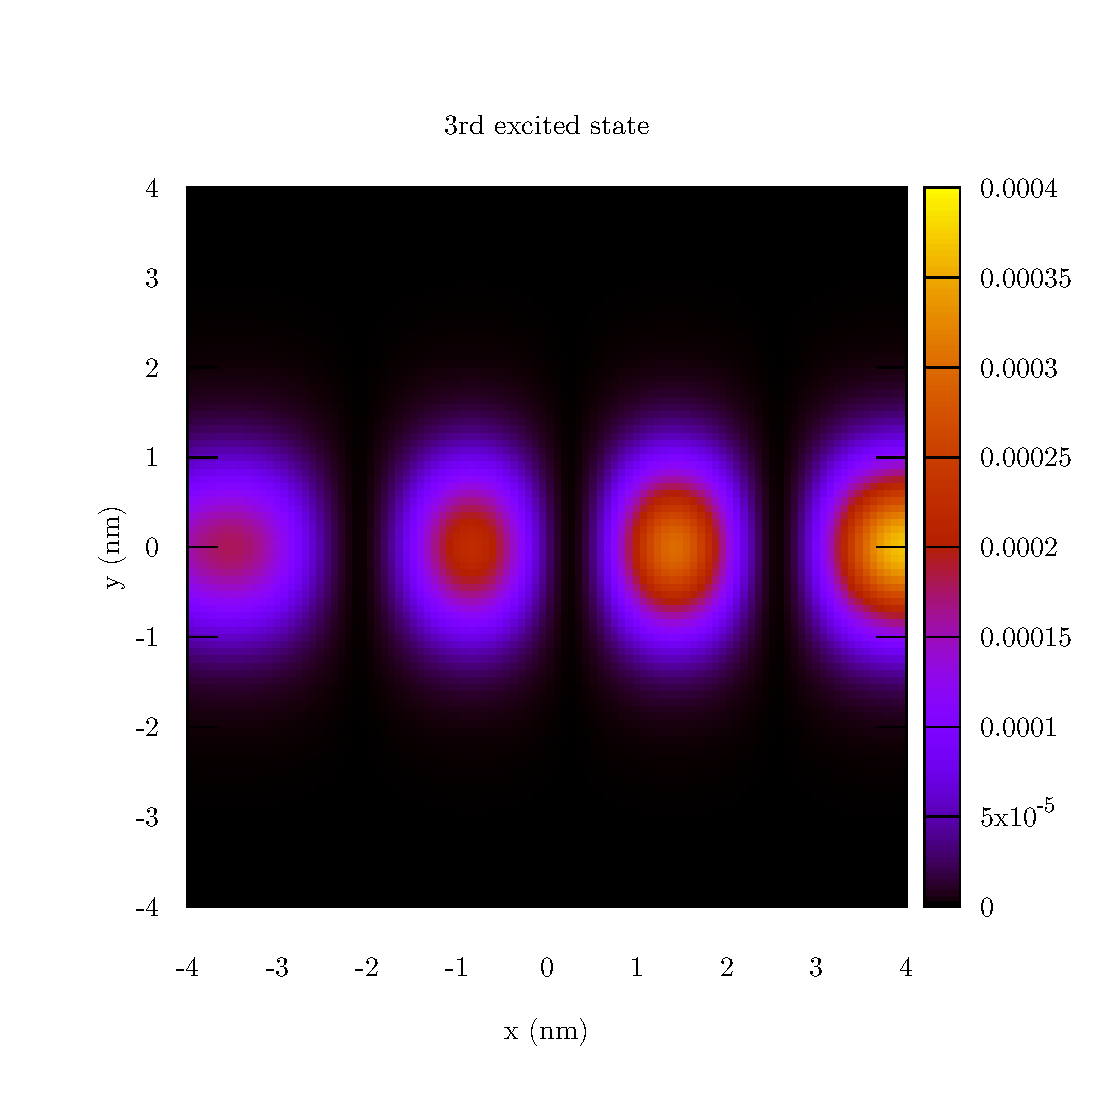
\includegraphics[width=\textwidth]{../plots/y_state_3.pdf}
		\caption{3rd excited state}
	\end{subfigure}
	\begin{subfigure}{.33\textwidth}
		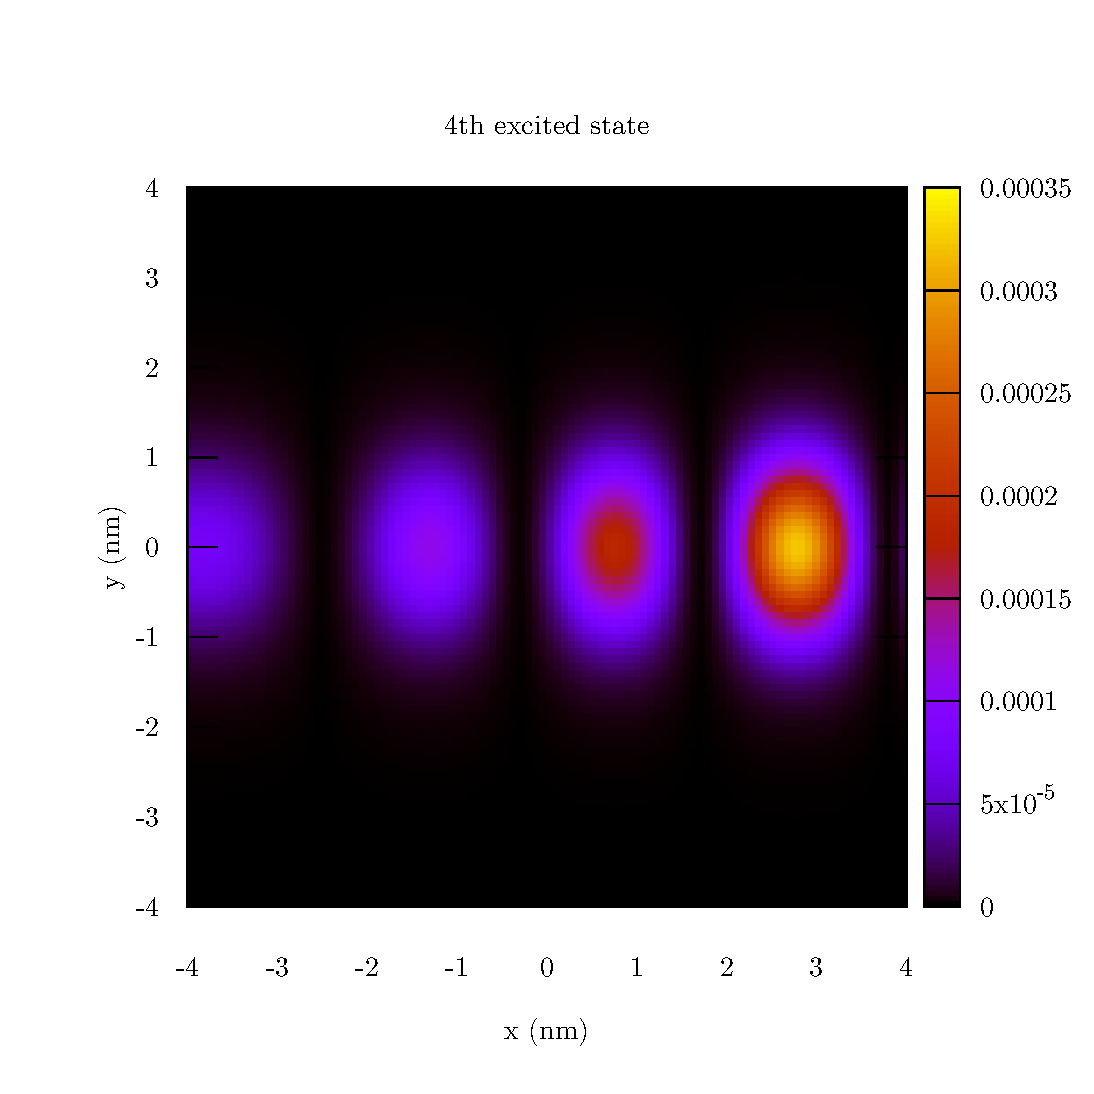
\includegraphics[width=\textwidth]{../plots/y_state_4.pdf}
		\caption{4th excited state}
	\end{subfigure}
	\caption{Probability densities of eigenstates composed from calculated coefficients for 2D harmonic oscilator where $ \hbar\omega_x=80 $ meV and $ \hbar\omega_y =360$ meV.}
\end{figure}

Achieved results are similiar to those aquired experimentaly. Here we can also observe multiple gaussian-like probability density dystibutions, where number of maximums is bigger for higher excited states.


\section*{Summary}

The problem of single electron in two dimentional parabolic potential has been solved using the Gallerkin method with gaussian base function set. The generalized eigen problem has been solved using the algorythms already implemented in \texttt{Eigen3} library. 

\end{document}
